\textbf{1-1} 如力图1-1-1，直角三角形ABC在铅垂平面内，斜边AC与水平边BC的夹角为$\alpha$，一质点从A点由静止出发，在重力作用下到达C点。当所循路径为从A经AB和BC时，从A到B需时 $t_{1}$，从B到C需时 $t_{2}$；当所循路径为AC时需时 $t_{3}$，假定质点拐折时不花费时间，且只改变速度方向而速度大小不变。

1. 为使循上述两条路径由 $A$ 到 $C$ 所需时间相等，即使 $t_1 + t_2 = t_3$，试问角 $\alpha$ 应为多大？

2. 设角 $\alpha$ 取上述值，设质点只能在三角形范围内沿竖直路径和水平路径从 $A$ 点到达 $C$ 点，显然有无穷多种选择。试问什么路径花费的时间最多？什么路径花费的时间最少？所需的最长时间与最短时间之比是多少？

\begin{center}
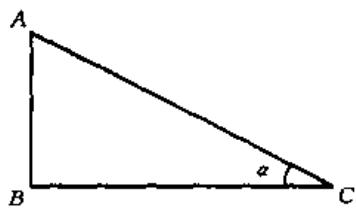
\includegraphics[width=0.3\textwidth]{figures/力图1-1-1.jpg}
\end{center}
\newpage

\textbf{1-2} 一质点以初速度 $v_{0}$ 作直线运动，所受阻力与其速度成正比。试求当质点速度减为 $\dfrac{v_0}{n}$ $(n > 1)$ 时，质点经过的距离与质点所能行经的总距离之比。

\vfill

\textbf{1-3} 一质点以初速度 $v_{0}$ 作直线运动，所受阻力与其速度的三次方成正比。试求质点速度和位置随时间的变化规律以及速度随位置的变化规律。

\vfill

\newpage

\textbf{1-4} 如力图1-4-1，在倾角为 $\theta$ 的山坡平面上有一门大炮，大炮相对于山坡的仰角为 $\alpha$，发射炮弹的初速为 $v_{0}$。试求炮弹着点的位置，并求能达到最大射程的仰角，忽略空气阻力。

\begin{center}
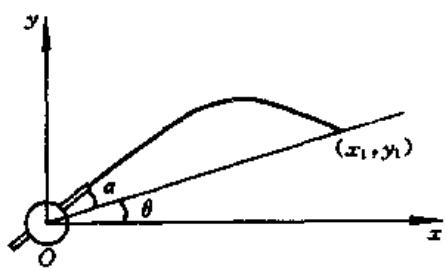
\includegraphics[width=0.3\textwidth]{figures/力图1-4-1.jpg}
\end{center}
\vfill

\textbf{1-5} 两质点在地面上同一地点以相同速率 $v_{0}$ 从不同抛射角抛出。试证明，当两质点的射程 $R$ 相同时，它们在空中飞行时间的乘积为 $\dfrac{2R}{g}$，忽略空气阻力。

\vfill

\textbf{1-6} 如力图1-6-1，位于地面的水枪与一竖直墙的垂直距离为 $d = 3.0\,\mathrm{m}$，墙高 $h = 4.0\,\mathrm{m}$。从水枪喷出初速恒定的水流，为使水流刚好能越过墙顶，试问水流从枪口喷出的初速 $v_{0}$ 的最小值以及水枪的仰角 $\alpha$ 各为多少？忽略空气阻力，重力加速度 $g$ 取 $10\,\mathrm{m/s^2}$。

\begin{center}
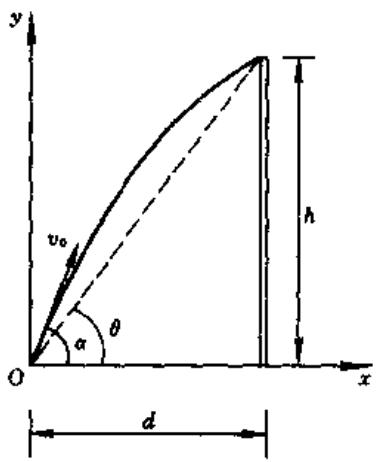
\includegraphics[width=0.3\textwidth]{figures/力图1-6-1.jpg}
\end{center}
\vfill

\newpage

\textbf{1-7} 如力图1-7-1，球1和球2均从同一点水平抛出，起抛点离水平地面的高度为 $H$。两球的水平初速分别为 $v_{1}$ 和 $v_{2}$ $(v_{1} > v_{2})$。球1抛出后刚好能越过位于 $x_{P}$ 处的竖直杆的顶端，并落于地面上的 $R$ 点，$R$ 点与 $O$ 点的距离为 $R$。球2抛出后落于地面，与地面作弹性碰撞，反弹后也刚好越过杆顶，并落在同一点 $R$。试求：1. 比值 $\dfrac{v_1}{v_2}$。2. 杆的位置 $x_{P}$。3. 杆的高度 $h$。

\begin{center}
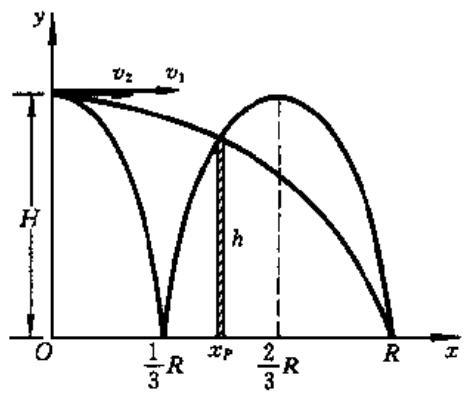
\includegraphics[width=0.3\textwidth]{figures/力图1-7-1.jpg}
\end{center}
\vfill

\textbf{1-8} 飞行物自地面以匀速 $v_{\mathrm{f}}$ 向上空垂直飞行。在地面离飞行物起飞点相距 $L$ 处发射一枚导弹，导弹与飞行物同时发射。导弹的速率 $v$ 为常值，且 $v > v_{\mathrm{f}}$，每一瞬时导弹均指向飞行物运动。

1. 试求导弹的飞行轨迹；

2. 试问导弹经多长时间击中飞行物。

\vfill

\newpage

\textbf{1-9} 圆柱体固定不动，其轴线与水平面垂直。很轻的不可伸长的柔软细线全部缠绕在圆柱体上且在同一水平面内，线末端系一小球，紧贴圆柱体表面。突然给小球一击，使之具有在水平方向并与圆柱体垂直的初速度 $\boldsymbol{v}$，于是缠绕的细线开始从圆柱体上解开。设解开过程中细线与圆柱体之间无相对滑动，且重力可略，即小球始终在水平面内运动。

试求：1. 小球的加速度。2. 小球的轨迹方程。

\vfill

\textbf{1-10} 细杆绕端点 $O$ 在平面内匀角速旋转，角速度为 $\omega$，杆上一小环（可看作质点）相对杆作匀速运动，相对速度为 $v$。设 $t = 0$ 时刻小环位于杆的端点 $O$。

1. 试证明小环的运动轨迹为阿基米德螺线。

2. 试求小环在任意时刻的速度和加速度。

3. 试用作图法定性画出小环加速度在自然坐标系中的两个分量（切向加速度和法向加速度）。

\vfill

\newpage

\textbf{1-11} 如力图1-11-1所示，质点 $A$ 和质点 $B$ 同时从 $A$、$B$ 两点出发，分别以速度 $v_{1}$ 沿 $AB$ 和以速度 $v_{2}$ 沿 $BC$ 作匀速直线运动，$BC$ 和 $AB$ 的夹角为 $\alpha$，开始时质点 $A$ 和质点 $B$ 相距为 $l$，试求两质点之间的最短距离。

\begin{center}
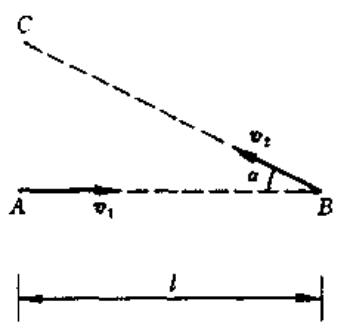
\includegraphics[width=0.2\textwidth]{figures/力图1-11-1.jpg}
\end{center}
\vfill

\textbf{1-12} 宽 $L$ 的河流，流速与离岸的距离成正比，已知两岸处的流速为零，河中心的流速为 $v_{0}$。一小船以恒定的相对速度 $v_{r}$ 垂直于水流从一岸驶向另一岸。在离岸 $\dfrac{L}{4}$ 处因故突然掉头，以相对速度 $\dfrac{v_{r}}{2}$ 垂直于水流驶回本岸。

试求：1. 小船的运动轨迹。2. 小船返回本岸时，所到处与原出发点的距离是多少。

\vfill

\newpage

\textbf{1-13} 如力图1-13-1，一条笔直的河流宽度为 $d$，河水以恒定的速度 $v_{0}$ 流动。小船从河岸的 $A$ 点出发，为了到达对岸的 $O$ 点，相对于河水以恒定的速率 $v^{\prime}$ $(v^{\prime} > v_{0})$ 运动，不论小船驶到何处，它的运动方向总是指向 $O$ 点。已知 $\overline{AO} = r_0$，$\angle AOP = \varphi_0$，试求小船运动的轨迹。若 $O$ 点刚好在 $A$ 点的对面（即 $\overline{AO} = d$），结果又如何？

\begin{center}
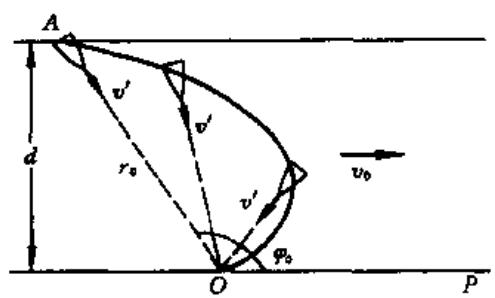
\includegraphics[width=0.3\textwidth]{figures/力图1-13-1.jpg}
\end{center}
\vfill

\textbf{1-14} 如力图1-14-1，轮子在水平面上以角速度 $\omega$ 作纯滚动，已知轮子的质心速度为 $v_{\mathrm{c}}$，试求轮边缘上任一点 $A$ 的绝对速度，$A$ 点的位置用 $\theta$ 角表示。

\begin{center}
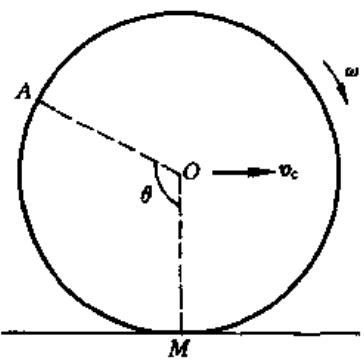
\includegraphics[width=0.3\textwidth]{figures/力图1-14-1.jpg}
\end{center}
\vfill

\newpage

\textbf{1-15} 如力图1-15-1，半径为 $R$ 的圆环静止不动，半径为 $r$ 的圆盘沿圆环内侧作无滑动的滚动，圆盘中心 C 点绕环中心 O 点的角速度恒为 $\Omega$。试求圆盘上与圆环相接触的 A 点相对圆环的加速度。

\begin{center}
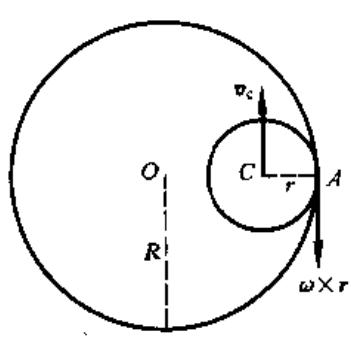
\includegraphics[width=0.2\textwidth]{figures/力图1-15-1.jpg}
\end{center}


